% !TEX encoding = UTF-8 Unicode
\documentclass{pclass}
\usepackage[utf8]{inputenc} % para linux y mac 
%\usepackage[latin1]{inputenc} % para windows

%DIFERENTES TIPOS DE LETRA
%\usepackage{palatino}
\usepackage{times}
\usepackage{subcaption}
\usepackage{textcomp}
\captionsetup{compatibility=false}


\begin{document}
\tipo{Grado}   % Grado o M\'aster
\titulopro{Segmentación de células en imágenes 3D con técnicas de machine learning}
\colaborador{Luis María Escudero Cuadrado\\Departamento de Biología Celular, Universidad de Sevilla}
\tutor{María José Jiménez Rodríguez}
\departamento{Matemática Aplicada I}
%\autores{Nombre 1}{Nombre 2}  % Dos autores
\autores{(ponente): Adrián López Carrillo}{{\ }}   % Un autor
\dia{27 de Septiembre de 2020 (v.1.1)}
\titulacion{Grado en Ingeniería Informática: Tecnologías Informáticas}

\hacerportada
	\makeatletter
\renewcommand*\l@section{\@dottedtocline{1}{0em}{2.5em}}
\renewcommand*\l@subsection{\@dottedtocline{2}{1.5em}{3.2em}}
\renewcommand*\l@subsubsection{\@dottedtocline{3}{4.3em}{3.2em}}
\makeatother

\renewcommand{\frontmatter}{\pagenumbering{Roman}}
%\frontmapertter

    \cdpchapter{Resumen}

En la actualidad existen microscopios que emplean técnicas ópticas para reconstruir imágenes 3D con una alta precisión. Gracias a esto los investigadores tienen a su alcance imágenes microscópicas de alta calidad para poder sacar conclusiones de ellas. Estas imágenes suelen requerir un procesado digital con el objetivo de discernir los elementos importantes del resto.

En este proyecto se abordará el problema de la segmentación de células en imágenes 3D. Para ello se usarán imágenes  cedidas por el Departamento de Biología Celular de la Facultad de Biología de la Universidad de Sevilla. En cada imágen hay decenas de células, todas en contacto con otras células sin espacio entre ellas.

El procesado digital de estas imágenes actualmente se hace de forma manual teniendo una duración de una a dos semanas, por lo que la automatización de este proceso conllevará un gran ahorro de tiempo.

Respecto a las técnicas usadas, este proyecto se centrará en el uso de redes neuronales para la segmentación de células. Se validará la efectividad del uso de redes neuronales y se estudiará qué tipo de red neuronal y arquitectura será mejor para esta tarea, teniendo en cuenta la exactitud de la segmentación y el coste computacional.

En el análisis de antecedenes se comprobará que la CNN (Convolutional Neural Network o Red Neuronal Convolucional) será con la que se obtienen mejores resultados en el reconocimiento de patrones en imágenes. También se verá que al diseñar una CNN con la arquitectura U-Net se obtienen buenos resultados.

Se probarán varios modelos de CNNs para la segmentación de células, esperándose el mejor resultado de la arquitectura U-Net.

Adicionalmente, se estudiará el uso de un preprocesado y postprocesado para aumentar la eficacia de la segmentación, así como un posterior mapeado a color de las células para ayudar a su visualización.

Esta herramienta estará disponible para el usuario final por medio de una imágen docker, para facilitar su distribución y que perdure el paso del tiempo.

%    \cdpchapter{Agradecimientos}

A nuestros alumnos y a nuestras alumnas.

	\tableofcontents % Índice de contenidos
 	\listoftables % Índice de cuadros
 	\listoffigures % Índice de figuras
% 	\lstlistoflistings %Índice de códigos

 \mainmatter
     \part{Introducci\'on}\label{introduccion}
     \newpage
	 \thispagestyle{empty} % empty
	 \mbox{}
 	 \chapter{Nacimiento del proyecto}\label{nacimiento}

Uno de los mayores intereses del autor de este proyecto en el mundo del software siempre ha sido el uso de técnicas de inteligencia artificial para resolver problemas actuales.

Aprovechando que cursaba la asignatura de Procesamiento de Imágenes Digitales con la profesora María José Jiménez Rodríguez para preguntarle si sabía de algún TFG en el que estuviesen involucradas imágenes y pudiese desarrollar una solución de inteligencia artificial. La principal motivación par esto era que nunca había trabajado con imágenes digitales en el ámbito de machine learning.

María José habló sobre un proyecto muy interesante dirigido por el investigador Luis María Escudero Cuadrado del Departamento de Biología Celular de la Universidad de Sevilla. Parte de este este proyecto consistía en procesar imágenes 3D de glándulas salivales tomadas por un microscopio confocal para obtener la segmentación de las células. Un punto importante era que este procesado fuese automático ya que se podría ahorrar mucho tiempo, por lo que estaban valorando el uso de técnicas de machine learning.

Tras ver que este proyecto era interesante se planeó una primera visita al Departamento de Biología Celular, siendo recibidos por Luis María Escudero, Pablo Vicente-Manuera y Pedro Gómez-Gálvez. En esta reunión se habló en más detalle sobre la investigación que realizaban y el problema que se iba a abordar en el TFG.

Estaban estudiando la arquitectura a nivel celular del tejido epitelial. El tejido epitelial es uno de los 4 tejidos animales básicos, por lo que gran parte del organismo está compuesto por éste. Aunque las células de este tejido siempre se han representado en forma de prisma (cuando las células están en el mismo plano) o en forma de tronco (cuando se produce un pliegue), han demostrado que en condiciones de curvatura adoptan forma de escutoide para estabilizar energéticamente el tejido. La forma geométrica escutoide fue descubierta por este grupo de investigación \cite{GomezGalvez2018}. En la figura \ref{fig:tejidoepitelial} se pueden ver las forma de prisma, tronco y escutoide.

\figura{1}{img/tejidoepitelial}{\textbf{a} Representación de las células del tejido epitelial cuando están en una estructura plana. Se suele representar en forma de prisma. \textbf{b} Representación de las células del tejido epitelial cuando se produce un pliegue. Se suele representar en forma de tronco. \textbf{c} Geometría propuesta caracterizada por tener al menos un vértice en un plano distinto al de sus dos bases. En la figura de arriba se ven dos elementos adyacentes con forma escutoide. En la figura de abajo se ven estos elementos por separado. Las células del tejido epitelial tendrían esta geometría. (Figura editada procedente de Gómez-Gálvez et. al 2018)}{fig:tejidoepitelial}{}

Para obtener un modelo visual del tejido epitelial empiezan utilizando un microscopio confocal del que obtienen un stack de imágenes 2D, consiguiendo así una imagen 3D. Esta imagen es procesada computacionalmente utilizando herramientas de MATLAB y Fiji (ImageJ) para conseguir una imagen con todas las células etiquetadas correctamente, proceso conocido como segmentación semántica. El resultado final sería una imagen en la que cada vóxel del fondo tiene valor 0 y los vóxeles pertenecientes a cada célula tienen valor $1,2,3...n$, donde $n$ es el nº de células en la imagen. Un ejemplo de dos capas de la imagen 3D original y la imagen etiquetada puede verse en la figura \ref{fig:ejemplo1_segmentacion}

\begin{figure}[ht]
\centering
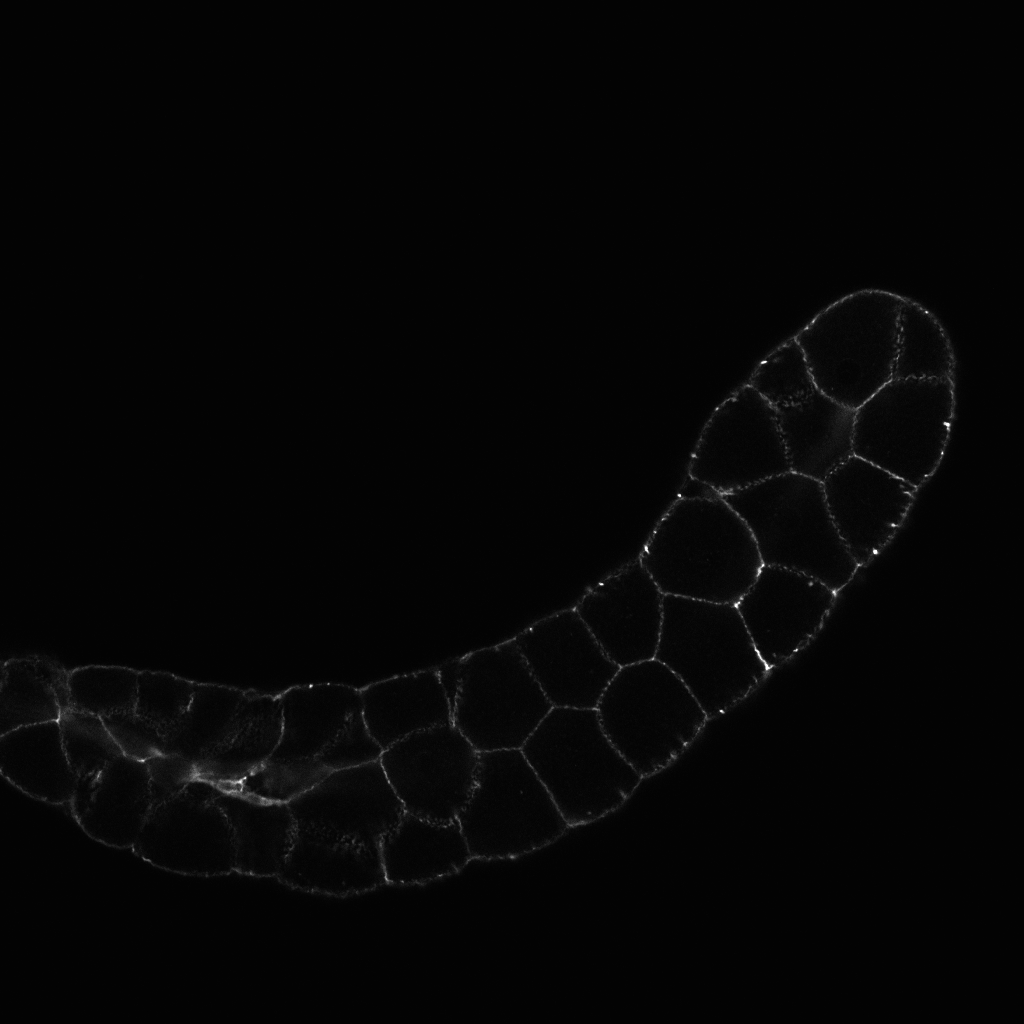
\includegraphics[scale=0.2]{img/raw 04_1a Z=77.png}
\vspace*{1mm}
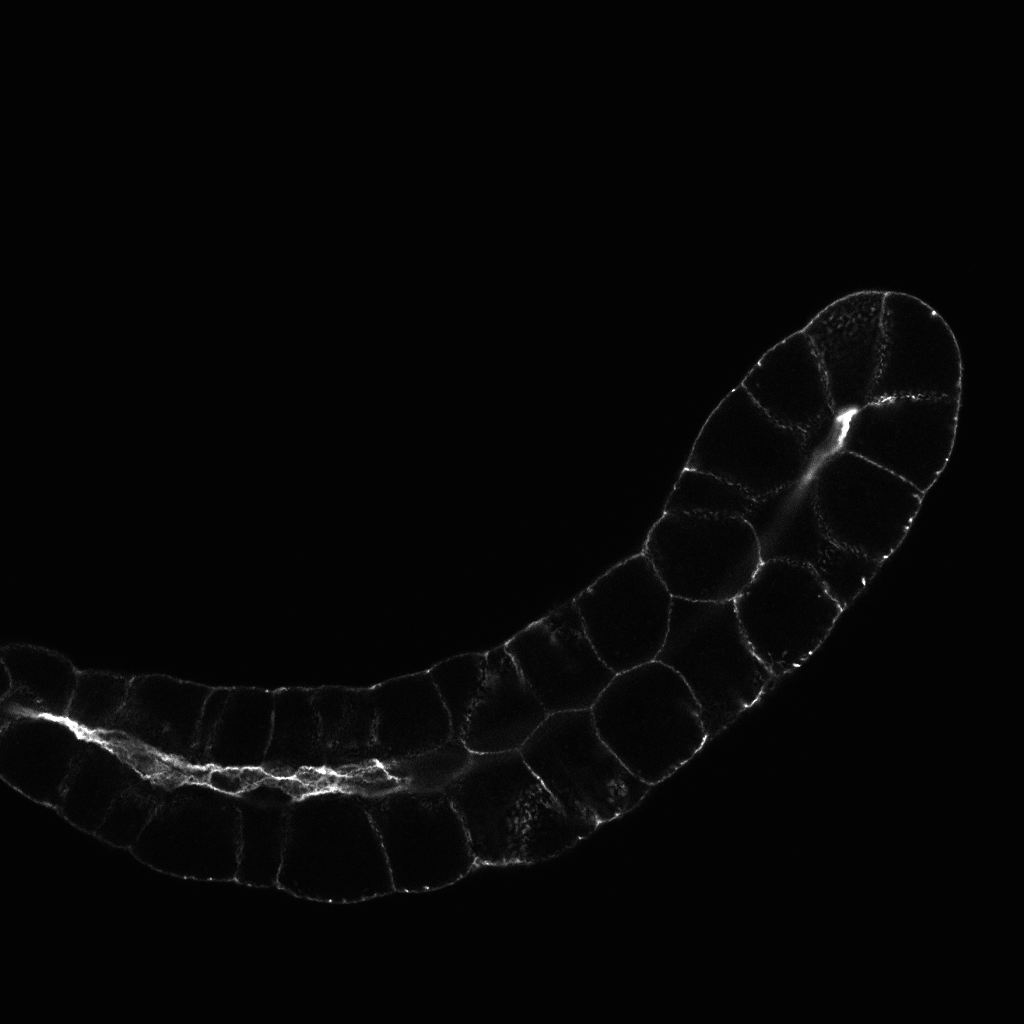
\includegraphics[scale=0.2]{img/raw 04_1a Z=100.png}
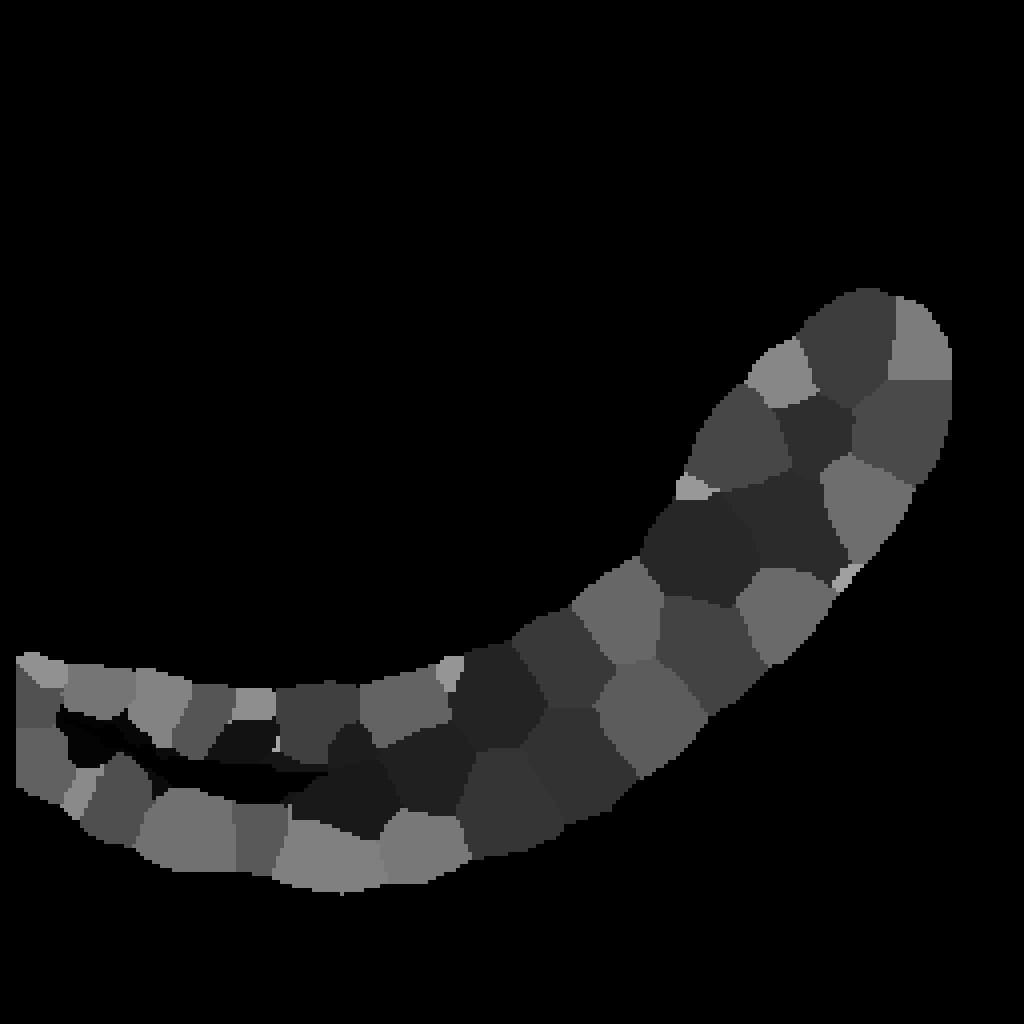
\includegraphics[scale=0.2]{img/target 04_1a Z=77.png}
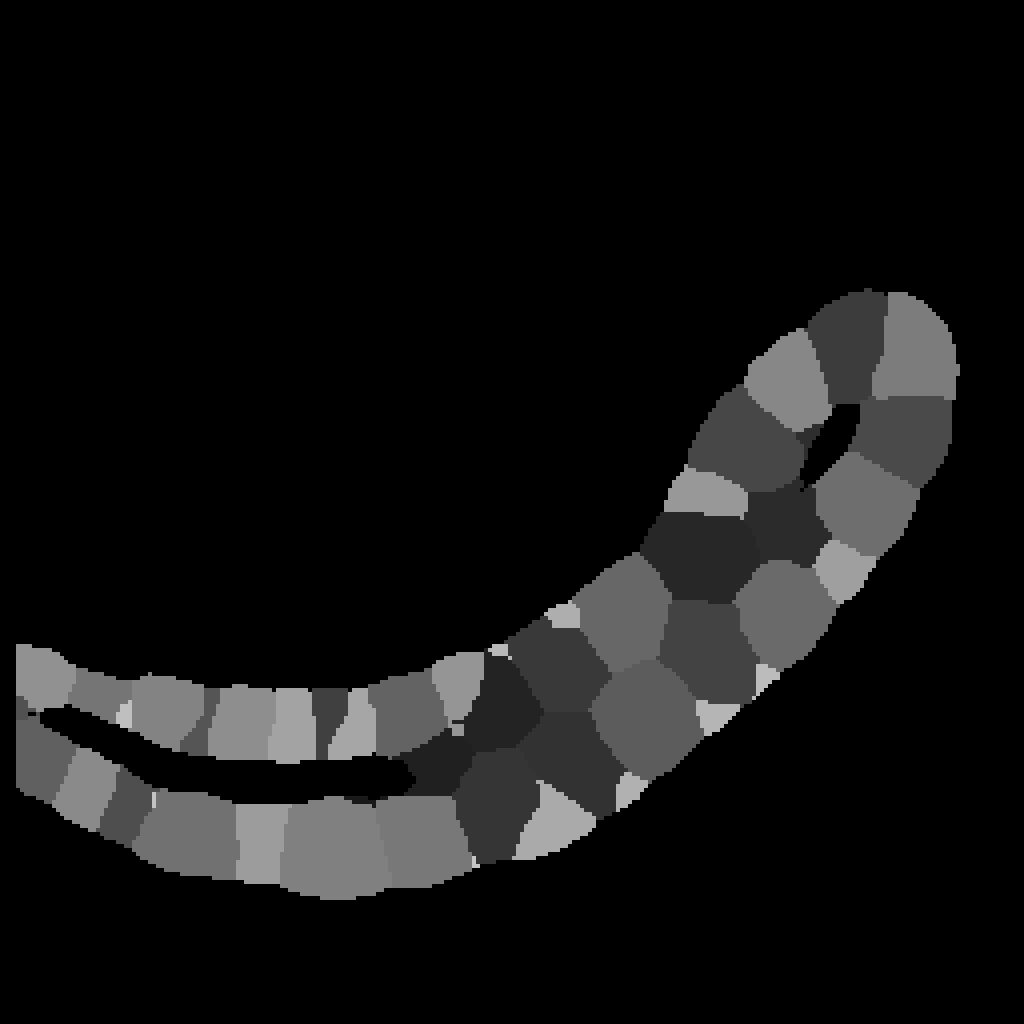
\includegraphics[scale=0.2]{img/target 04_1a Z=100.png}
\caption{Esta figura muestra el resultado de aplicar el procesado a la imagen 3D de una glándula salivar de Drosophila (un género de moscas), obtenida por microscopía. La imagen tiene las dimensiones $1024*1024*234$, seleccionándose para su representación Z=77 y Z=100. En la primera fila se muestra la imagen obtenida por microscopía y la segunda fila se muestra la obtenida al aplicar segmentación a las células. En la primera columna se muestra la capa Z=77 y en la segunda la capa Z=100.}\bigskip
\label{fig:ejemplo1_segmentacion}
\end{figure}

Pasar de la primera fila de la figura \ref{fig:ejemplo1_segmentacion} a la segunda fila es un proceso que puede llevar hasta una semana ya que se quiere conseguir un etiquetado perfecto. Esto provoca que se invierta mucho tiempo en una tarea repetitiva y poco interesante y se reste tiempo de las tareas de interés científico. Querían reducir el tiempo necesario para la segmentación y para ello pensaron que sería buena idea recurrir a técnicas de machine learning. Sería el objetivo principal del TFG, por tanto, obtener una segmentación automática que redujera el tiempo de segmentación manual, siendo lo ideal obtener directamente la segmentación perfecta.
     \chapter{Objetivos}

Este proyecto comenzó con la idea de reducir el tiempo necesario para tener una segmentación correcta de las células, por lo que ese será el objetivo principal. En las etapas iniciales del proyecto, tal y como se verá en el capítulo \ref{sec:nosetuvoencuenta} hubo un cambio de rumbo en el alcance del proyecto, es por ello que se añadió un objetivo relacionado con el coste de computación. En definitiva, los objetivos son los siguientes:

\begin{enumerate}
\item Utilizar técnicas de machine learning para desarrollar un modelo que, a partir de una imagen 3D de tejido epitelial, calcule una segmentación de las células lo más cercano posible a una segmentación perfecta.
\item Debido a que especies con distintos fenotipos pueden presentar glándulas con distinta morfología a nivel celular, es útil la posibilidad de poder entrenar un modelo con distintos datasets.
\item Debido a las dificultades encontradas en el primer acercamiento al problema, hacer que el proyecto funcione correctamente con una capacidad de computación limitada.
\item Debido a que el proyecto será utilizado por personal del ámbito científico y no tecnológico, hacer que el proyecto sea de uso e instalación sencilla.
\end{enumerate}
	 \part{Organizaci\'on del Proyecto}\label{organizacion}
	 \newpage
	 \thispagestyle{empty} % empty
	 \mbox{}	 
	 \chapter{Planteamiento inicial}\label{planinicial}

\section{Plan inicial}\label{sec:planinicial}

El primer enfoque para abordar este proyecto fue utilizar herramientas actuales de machine learning para la segmentación semántica de las imágenes provistas y, a partir de los resultados obtenidos, investigar cómo mejorar la segmentación. Sin embargo esto no fue posible debido a la alta resolución de las imágenes provistas y al limitado acceso a hardware de alto rendimiento. Por ello se ideó un plan inicial en el que se construía una herramienta que tuviese menor requisito de hardware. La mayor limitación era por la VRAM necesaria, por lo que se pensó en utilizar Apache Spark \cite{apachespark} para aprovechar HDD y RAM.

En este primer plan se dividieron las tareas en fases, siendo la fase 0 realmente un proceso de iniciación, necesaria para planificar el resto de las fases.

\begin{itemize}
\item[\textbf{Fase 0}] Estudio previo. Investigar las soluciones actuales al problema o problemas similares, las posibles técnicas de machine learning a usar en este proyecto y tecnologías para implementarlas.
\item[\textbf{Fase 1}] Aprender a implementar una CNN en Python. Usar datos de prueba para familiarizarme con las tecnologías a usar en este proyecto. Se explica en más detalle por qué usar CNN en la sección \ref{sec:archs}. El uso de Python se explica en la sección \ref{subsec:language}.
\item[\textbf{Fase 2}] Implementar, entrenar y probar una o más CNN.
\item[\textbf{Fase 3}] Analizar resultados obtenidos.
\item[\textbf{Fase 4}] Investigar sobre mejoras pre y post procesado.
\item[\textbf{Fase 5}] Realizar estas operaciones usando Apache Spark. Framework que facilita trabajar con datos a gran escala aprovechando HDD y RAM.
\item[\textbf{Fase 6}] Hacer que el entrenamiento y la inferencia sean usables por un usuario.
\end{itemize}

\section{Nueva metodología}\label{sec:metodologia}

Gracias a la investigación inicial realizada en la \textbf{Fase 0} se pudo definir el resto de fases del plan inicial, aunque no se tuvieron en cuenta varios factores que se empezaron a ver en la \textbf{Fase 1} y \textbf{Fase 2}. Esto provocó que se tuviese que realizar un ajuste en el plan inicial. 
Lo que no se tuvo en cuenta fue:

\begin{itemize}
\item Las fases 2, 3 y 4 deben ser fases iterativas. Cada vez que se obtengan resultados hay que estudiarlos y hacer cambios para mejorar los resultados.
\item No se tiene en cuenta el rendimiento de los algoritmos utilizados ni los cuellos de botella.
\item Se quiere usar Spark con la premisa de aprovechar la RAM o el HDD cuando la VRAM se agote, pero esto no es viable ya en la VRAM se tiene que poder almacenar toda la información necesaria para ejecutar cada algoritmo.
\end{itemize}

Por todo ello, se buscó información sobre una metodología adecuada. El capítulo 11 del libro Deep Learning \cite{Goodfellow2016} habla sobre una metodología práctica para la aplicación de técnicas en deep learning. Esta metodología se centra en utilizar feedback del sistema construido en cada iteración para modificar el sistema acorde a los objetivos. Los pasos a seguir propuestos por esta metodología son:

\begin{enumerate}
\item Determinar las metas. Qué métrica usar como error y un valor de la métrica aceptable como objetivo.
\item Establecer lo antes posible un sistema completo que pueda dar un valor para dicha métrica.
\item Utilizar herramientas adecuadas para determinar cuellos de botella en el rendimiento. Comprobar qué componentes están dando peores resultados en el sistema y comprobar si los resultados negativos son debidos a overfitting, underfitting, a un fallo con los datos o en el software.
\item Hacer cambios de forma a los datos, ajuste de hiperparámetros o cambiar algoritmos con el objetivo de mejorar la métrica usada. Volver al punto 3.
\end{enumerate}

Estos pasos se resumirán como ``desarrollo del sistema" y constituirá la mayor parte del proyecto.
\newpage
\section{Plan seguido}\label{sec:planactualizado}

\begin{itemize}
\item[\textbf{Fase 0}] Estudio previo. En esta fase se investigará sobre artículos de segmentación celular y se aprenderá sobre machine learning y las tecnologías necesarias para llevar a cabo resultados similares aplicados al problema actual.
\item[\textbf{Fase 1}] Desarrollo del sistema. Aplicar la metodología de la sección \ref{sec:metodologia}.
\begin{enumerate}
\item Determinar metas con métricas.
\item Sistema inicial.
\item Usar herramientas para determinar cuellos de botella en el rendimiento.
\item Cambios en el sistema.
\item Si no se ha alcanzado el valor objetivo de la métrica, volver al punto 3.
\end{enumerate}
\item[\textbf{Fase 2}] Mejoras de usabilidad. Que el proyecto sea usable por un usuario.
\item[\textbf{Fase 3}] Cierre. Terminar de escribir la memoria con los resultados obtenidos, las conclusiones, tabla de tiempos y manual de usuario.
\end{itemize}

	 \chapter{Costes}\label{costes}


	 \part{Desarrollo}\label{desarrollo}
	 \newpage
	 \thispagestyle{empty} % empty
	 \mbox{} 
	 \chapter{An\'alisis de antecedentes y aportaci\'on realizada}\label{analanteced}

%En este capítulo se hará una breve twintroducción a las redes neuronales, se justificará el uso del tipo de red neuronal CNN para tratamiento de imágenes así como el de la arquitectura CNN U-Net para la segmentación de células.

\section{Red Neuronal}\label{sec:redneuronal}
En esta sección se hará una breve introducción a las redes neuronales artificiales, compuesta por neuronas artificiales. Primero se describirá qué es una neurona artificial y se definirán 3 tipos: perceptrón, sigmoide y unidad lineal rectificada (ReLU). Después se hablará sobre el entrenamiento. Por último se hablará sobre los componentes de una red neuronal y a qué llamaremos modelo.
\subsection{Partes de una Red Neuronal}\label{subsec:nn_partes}

\subsection{Neurona artifical}\label{subsec:neurona_artificial}

Una neurona artificial es un componente básico en una red neuronal artifical. Un primer modelo fue introducido por Warren McCulloch y Walter Pitts en 1943, a partir del cual se han hecho mejoras a lo largo de los años. \cite[Chapter~1]{Rojas1996}

En la figura \ref{fig:generic_computing_unit} se puede ver una neurona artifical genérica con la que pueden ser descritas los distintos tipos que se verán en esta sección.

\figura{1}{img/Rojas1996_p31_computing_unit}{Neurona artificial genérica}{fig:generic_computing_unit}{}

Siendo:
\begin{itemize}
\item $ (x_1, x_2, ...,x_n) $ el vector de entrada.
\item $ (w_1, w_2, ...,w_n) $ el vector de pesos.
\item $ g $ la función de integración, encargada de reducir el vector de entrada a un único valor.
\item $ f $ la función de activación, encargada de producir la salida de este elemento.
\end{itemize}

Se puede simplificar la representación al asumir que siempre se usará $ \sum $ como función de integración. Será común ver una representación como \ref{fig:neurona_artificial_no_bias} en la que $ f $ indicará la función de activación.

\figura{1}{img/neurona_artificial_no_bias}{Representación simplificada de una neurona artificial}{fig:neurona_artificial_no_bias}{}

\subsubsection{Perceptrón}\label{subsubsec:perceptron}

Fue propuesto inicialmente por Frank Rosenblatt en 1958 y perfeccionado por Minsky y Papert en la década de de 1960 \cite[p.~55-56]{Rojas1996}.
Su diseño está inspirado en las neuronas como bloque elemental en el funcionamiento del cerebro. 

El perceptrón es una unidad de computación con un umbral $ \theta $ el cual, al recibir un vector de entrada de tamaño $ n $ y dado un vector de pesos de tamaño $ n $, devuelve 1 si $ \sum_{i=1}^{n} w_i x_i \geq \theta $ y 0 en otro caso.\cite[p.~60]{Rojas1996}.

Para entender de forma intuitiva esta definición podemos tomar un ejemplo en el que $ n = 2, w_1 = 0.5, w_2 = 2, \theta = 1 $. En la figura \ref{fig:percep_graf_repr} se puede ver la línea $ 0.5x_1 + 2x_2 = 1 $ y los puntos $ p_1=(1;1), p_2=(-2;1.4) $ y $ p_3=(-0.4;-1) $. Se puede ver cómo $ p_1 $ y $ p_2 $ están por encima de la línea, por lo que devuelven 1 y $ p_3 $ por debajo, por lo que devuelve 0.

\figura{0.5}{img/percep_repr_graf}{Representación de todos los valores del vector de entrada}{fig:percep_graf_repr}{}

Si se despeja $x_2$ en la fórmula $ w_1 x_1 + w_2 x_2 = \theta $, se obtiene la ecuación de la recta $ x_2 = \frac{\theta}{w_2} - \frac{w_1}{w_2}x_1 $. Se puede intuir cómo al modificar el valor de $ \theta $ la línea se mueve de forma vertical, así cómo $ w_1 $ afecta a la pendiente y $ w_2 $ afecta a ambos aspectos.\\

Como se verá más adelante, entrenar una red neuronal implica actualizar los pesos, por lo que será importante representar las neuronas artificiales de forma que se pueda modificar $ \theta $ al modificar un peso. Tomando como base la representación de una neurona artificial vista en \ref{fig:neurona_artificial_no_bias}, se toman las siguientes consideraciones:\\

\begin{itemize}
\item Al vector de entradas se le añade un elemento de valor constante 1, siendo ahora de tamaño $ n+1 $.
\item Al vector de pesos se le añade un elemento de valor inicial $ -\theta $, siendo ahora de tamaño $ n+1 $. A este valor se le llamará \textit{bias}.
\item Se usara como función de activación la función escalón unitario.
\end{itemize}

\figura{1}{img/Perceptron}{Perceptrón. Mostrando el bias como entrada.}{fig:perceptron}{}

\subsubsection{Sigmoide}\label{subsubsec:sigmoide}

La función sigmoide como función de activación es una función no lineal usada principalmente en redes neuronales prealimentadas (feedforward neurals networks), que son las que usaremos en este proyecto. Es una función real, acotada y diferenciable (a diferencia de la usada en el perceptrón). Su definición es la siguiente relación \cite{nwankpa2018activation}:

\begin{equation}
 f(x) = \frac{1}{1+e^{-x}}
\end{equation}

\subsubsection{Unidad Lineal Rectificada (ReLU)}\label{subsubsec:relu}

La unidad lineal rectificada (ReLU) fue propuesta como función de activación en 2010 por Nair y Hinton \cite{Nair2010} y desde entonces ha sido la más usada en aplicaciones de aprendizaje profundo (deep learning, DL). Si se compara con la función de activación Sigmoide, ofrece un mejor rendimiento y es más generalista \cite{nwankpa2018activation}.

\begin{equation}
 f(x) = max(0, x)=\left\{\begin{matrix}
 x_i & $si $ x_i \geq 0 \\ 
 0 & $si $ x_i < 0
\end{matrix}\right.
\end{equation}

\subsection{Algoritmos de aprendizaje}\label{subsec:learning_algos}
\section{Red Neuronal Convolucional}\label{sec:cnn}
\section{Reto ImageNet}\label{sec:imagenet}
\section{Arquitectura U-Net}\label{sec:unet}
     \chapter{Datos de entrada}\label{requisitos}

Los datos iniciales son 20 ficheros con formato hdf5, cada uno contiene la siguiente:

\begin{itemize}
\item \textbf{imageSequence}: Imagen inicial con la forma $ (Z1, 1024, 1024) $
\item \textbf{imageSequenceInterpolated}: Imagen incial interpolada, ahora con la forma $ (Z2, 1024, 1024) $. Siendo $ Z2 > Z1 $. 
\item \textbf{labelledImage3D}: Resultado de etiquetar correctamente la imagen inicial interpolada $ (Z2, 1024, 1024) $.
\item \textbf{centroidOfRois}: Coordenadas del centroide de cada célula.
\item \textbf{usedZScale}: Valor usado en la interpolación.
\end{itemize}

A continuación se analizarán las imágenes \textbf{imageSequenceInterpolated} y \textbf{labelledImage3D}.

\subsubsection{imageSequenceInterpolated}

El tipo usado para almacenar el valor de cada vóxel es \textit{f8} que, según la documentación de numpy es el equivalente a un número de 64-bit float.

Se han comprobado los valores máximo y mínimo de las 20 imágenes y estos son los resultados:

\cuadro{|r|c|c|c|c|c|c|c|c|c|c|c|c|c|c|c|c|c|c|c|c|}{Valores mínimo y máximo de los píxeles de las imágenes de entrada.}{tab:prueba}{
35.0 & 32.0 & 33.0 & 0.0 & 31.0 & 24.0 & 19.0 & 0.0 & 0.0 & 24.0 \\ 
4095.0 & 4095.0 & 4095.0 & 65535.0 & 4069.0 & 4095.0 & 4095.0 & 65535.0 & 65535.0 & 4095.0 \\
\hline
22.0 & 22.0 & 23.0 & 30.0 & 31.0 & 30.0 & 25.0 & 30.0 & 23.0 & 19.0 \\
4095.0 & 4095.0 & 4095.0 & 4095.0 & 4095.0 & 4095.0 & 4095.0 & 4095.0 & 4095.0 & 4095.0 \\
}

Se ha analizado el histograma de una imagen para entender mejor la distribución de valores. Podría ser que se pudiera simplificar el nº de valores distintos que tiene la imagen para aumentar el rendimiento. La imagen analizada tiene $ 32 $ de valor mínimo y $ 4095 $ de valor máximo.

En la figura \ref{fig:histogram1} se puede ver un histograma en el que en el eje $ x $ representa el valor de un píxel y el eje $ y $ representa el nº de píxeles con ese valor. En esta figura se puede comprobar que los valores están concentrados en el rango $ [0,500] $, pero da la impresión de que no hay ningún elemento en el resto de valores. Para obtener una mejor visualización del resto en la figura \ref{fig:histogram2} se puede ver otro histograma con el eje $ y $ limitado a 4000, donde se aprecia los distintos valores que un píxel puede tomar. 

\figura{0.8}{img/histograma1}{Histograma de todos los valores}{fig:histogram1}{}
\figura{0.8}{img/histograma2}{Histograma de todos los valores con el eje y limitado a 4000}{fig:histogram2}{}
     \chapter{Esquema general}\label{requisitos}

En este capítulo se describirá el flujo por el que pasan los datos suministrados hasta dar lugar a la segmentación objetivo, sin entrar en detalles sobre la las herramientas usadas en la implementación.

\subsubsection{Sistema inicial}

\figura{1.1}{img/diseno-sistema-inicial}{Diseño del sistema inicial.}{fig:diseno-sistema-inicial}{}{Diseño Sistema inicial.}

En la figura \ref{fig:diseno-sistema-inicial} se muestra un esquema general sobre el sistema inicial, explicado en más detalle en el capítulo \ref{initial_system}. 

Los dos primeros recuadros (azules) muestran los datos de entrada y el preprocesado necesario para que puedan ser utilizados en el entrenamiento.

La etapa de preprocesado no requerirá un uso intensivo de GPU, por lo que podrá realizarse en cualquier máquina. En este caso se usará la máquina local ya que la máquina en la nube es más costosa de utilizar.

En esta etapa se preparán los datos con 4 objetivos:
\begin{enumerate}
\item Reducir la resolución de la imagen de entrada, reduciendo así la memoria necesaria para almacenarla en GPU.
\item Generar las imágenes etiquetadas correctamente para tenerlas como objetivo.
\item Reducir el tamaño de los archivos resultantes, ya que estos serán usados en servicios cloud y tendrán que ser subidos y descargados con frecuencia.
\end{enumerate}

Tras esto, se generarán nuevos archivos hdf5 y se subirán a un disco duro virtual, al cual se accederá por un Notebook. Las imágenes de entrada podrán ser usadas como entrada en el modelo seleccionado, cuya salida será una segmentación de células con espaciado.

En el recuadro siguiente (naranja), se muestra el proceso que se lleva a cabo durante el entrenamiento de un modelo. Como ya se mencionó en el capítulo \ref{cloudcomputing} este proceso deberá realizarse con una GPU de alto rendimiento, por lo que en este proyecto se utilizará una máquina en la nube. Antes de comenzar este proceso los datos ya habrán sido cargados en un disco duro virtual. Se dividirá el dataset en $ 70\% $ entrenamiento, $ 15\% $ validación y $ 15\% $ test.


%Se utilizará un DataLoader, encargado de leer el dataset y realizar el preprocesado conveniente. Será importante normalizar los datos de entrada para que tengan un valor en rango $ [0, 1] $, esto se hará siempre. Adicionalmente, se probarán distintas técnicas como estandarizar el histograma, o \textit{data augmentation}. Al etiquetado objetivo no se le aplicará normalización ni estandarización, sólo se le aplicará \textit{data augmentation}. Al ser importante que la segmentación de la imagen etiquetada siga siendo correcta, al aplicar \textit{data augmentation} no se deformará la imagen.


%En el entrenamiento se usará un \textit{batch} de datos, se harán pruebas con valores en el rango $N\epsilon[1,4]$. Durante cada \textit{epoch}, tanto la predicción obtenida como la imagen con el etiquetado perfecto se transformarán con el \textit{one-hot encoding}, lo que les dará el formato $(N, C)$, donde $N$ es el tamaño del \textit{batch} y $C$ el nº de clases, que siempre será $C=2$. Esta disposición de datos transforma cada imagen en 2 vectores, uno por cada clase, lo cual hará que sea muy eficiente calcular diferencias entre la predicción y la imagen con etiquetado perfecto. Para calcular estas diferencias está la función de pérdida, que tendrá un valor bajo si hay poca diferencia y alto si hay mucha diferencia. El objetivo de cualquier algoritmo de optimización será disminuir esta función de perdida. Para la función de pérdida se probarán \textit{Dice Loss} y \textit{Cross Entropy Loss} con pesos. 

El valor dado por la función de pérdida con los datos de entrenamiento se usará en la \textit{backpropagation} para calcular los gradientes los cuales se usarán para optimizar los pesos con el optimizador Adam. El valor dado por la función de pérdida con los datos de validación será el que determine si el modelo ha mejorado de forma programática. Si el modelo no mejora al disminuir la pérdida significará que habrá que cambiar la función de pérdida.

El último recuadro de la figura \ref{fig:diseno-sistema-inicial} (en verde) muestra el proceso de inferencia. Se utilizará como mejor modelo aquél que haya obtenido una menor pérdida de validación durante el entrenamiento. Por ejemplo, si se entrena durante 100 iteraciones y en la iteración 89 se obtuvo la menor pérdida de validación, se utilizará el modelo entrenado durante esta iteración y se ignorarán las iteraciones posteriores. Tras realizar el entrenamiento completo se usarán los datos de test para obtener predicciones y se analizarán con la intersección sobre unión (\textit{intersection over union} o \textit{IoU}, con apoyo de la representación visual del resultado.

\subsubsection{Sistema final}
\figura{1.1}{img/diseno-sistema-final}{Diseño del sistema inicial.}{fig:diseno-sistema-final}{}{Diseño Sistema Final.}

En la figura \ref{fig:diseno-sistema-final} se muestra el diseño final del sistema tras aplicar todas las mejoras descritas en los capítulos siguientes.

Antes de utilizar la imagen original reescalada como entrada de la CNN, se han añadido dos pasos:
\begin{enumerate}
\item Normalización por unidad tipificada. Descrita en el capítulo \ref{znormalization}, este proceso es necesario reducir las diferencias de intensidad de los vóxeles y así facilitar el reconocimiento de patrones estructurales por la CNN. 
\item Data augmentation. Descrito en el capítulo \ref{data_augmentation}, este proceso es necesario para aumentar el nº de ejemplos de entrenamiento y reducir el sobreajuste.
\end{enumerate}

Además, se ha cambiado la arquitectura U-Net por una completa, como se verá en el capítulo \ref{full_unet}. La arquitectura del sistema inicial era temporal, pensada sólo para hacer iteraciones rápidas.

También se ha cambiado la función de pérdida por la pérdida DICE, como se verá en el capítulo \ref{loss_function}. Utilizar una función de pérdida que represente correctamente el error del problema a tratar es algo esencial, de no ser así la pérdida obtenida durante el entrenamiento calculará un error carente de interés.

Por último, se ha implementado la precisión mixta (capítulo \ref{apex}) para reducir la memoria y el tempo necesarios durante el entrenamiento e inferencia. Esto hará que en algunas operaciones se utilice un tipo de dato de 16 bits en vez de uno de 32 bits.
     \chapter{Implementación}\label{implementacion}

En este capítulo se mostrarán las tecnologías utilizadas para llevar a cabo el diseño deseado.

\section{Lenguaje y framework}\label{sec:language_framework}

El proyecto se ha desarrollado completamente en lenguaje de programación Python 3.7 y el framework PyTorch 1.6 \cite{Paszke2019}.

La elección del lenguaje Python es sencilla: los frameworks más utilizados en deep learning pueden ser usados en Python. Con una búsqueda rápida en GitHub bajo los términos "deep learning", "machine learning" y "neural network" se puede ver que los frameworks más populares pueden ser usados en Python.
\begin{itemize}
\item TensorFlow con 148k estrellas.
\item Keras con 49.4k estrellas.
\item PyTorch con 41.5k estrellas.
\item Caffe con 30.8k estrellas
\end{itemize}

Además, tal y como se muestra en el índice TIOBE \cite{Tiobe2020}, Python es el tercer lenguaje de programación con mejor puntuación teniendo en cuenta su presencia en los buscadores web.

Aún así Python tiene se su velocidad. Es lento cuando se compara con lenguajes como C y esto se debe principalmente a 2 motivos:
\begin{enumerate}
\item Es interpretado, no compilado. Al compilar un programa escrito en un lenguaje compilado el compilador optimiza el programa con una multitud de técnicas, como el desenrollado de bucles, que elimina o reduce las instrucciones de control de un bucle. En Python el intérprete sólo accede a la instrucción a realizar, no realiza ninguna tarea de optimización.
\item Es de tipado dinámico. Esto quiere decir que el intérprete no sabe de qué tipo es una variable hasta que intenta acceder a ella, por lo que antes de acceder a su valor debe comprobar el tipo de variable. Esto hace que las variables en Python sean fáciles de declarar y asignar, pero reduce el rendimiento.
\end{enumerate}

Estas desventajas se pueden reducir gracias a que Python tiene la capacidad de llamar a subrutinas en C o C++. Prácticamente todos los frameworks en los que se realizan operaciones con un alto coste computacional tienen la parte crítica de su código escrita en C o C++.

En el ecosistema de Python, la base matemática para cualquier framework que haga operaciones matriciales es NumPy \cite{VanDerWalt2011}, ya que añade soporte para arrays de n dimensiones y una gran multitud de operaciones de forma eficiente.

Todos los frameworks populares de Python son una buena elección, ya que todos tienen \textit{bindings} a lenguajes de bajo nivel compilados, pero con la facilidad de uso de Python. Aunque Tensorflow puede ser difícil de utilizar, cuenta con Keras, que es un framework desarrollado por encima que abstrae muchas operaciones. Pytorch, basado en Torch, también ofrece un fácil uso y buen rendimiento.

\section{Preprocesado local}\label{sec:local_preprocessing}

El primer paso a realizar es preparar los datos, para ello se han usado las siguientes librerías:

\begin{itemize}
\item \textbf{scikit-image} \cite{Walt2014}. Es una librería de procesamiento de imágenes. Se ha usado para encontrar los bordes de la imagen con etiquetado multiclase sin espaciado entre células. Esta imagen no podía ser usada directamente en el entrenamiento de la CNN, por lo que se ha seguido la estrategia de encontrar los bordes de cada célula con la función \textit{(segmentation.search\_boundaries())} \cite{Wolny2020}, después de encontrar los contornos se substraen de la imagen original y se cambian todas las etiquetas a 1, consiguiendo así un espaciado entre células, tal y como se indica en \cite{Falk2019}. También se ha usado esta librería (\textit{measure\_label()}) para asegurarnos de que el nº de células no varía al realizar las operaciones de preprocesado (por ejemplo, podría ser que dos células con etiqueta 1 eliminaran el espacio entre sí, convirtiendose en la misma instancia de célula).
\item \textbf{SciPy} \cite{Virtanen2020}. Contiene diversos módulos con algoritmos útiles en el ámbito científico. En el submódulo \textit{ndimage} se pueden encontrar los algoritmos relativos al procesamiento de imagen. Se ha utilizado la función \textit{ndimage.zoom()} para reescalar las imágenes de entrada, haciendo que ocupen menos memoria y sea viable usarlas para el entrenamiento.
\item \textbf{h5py} \cite{Collette2013}. Aporta una interfaz para trabajar con el formato de datos HDF5 \cite{HDFGroup20002010}, útil para usar en python ficheros generados en programas como MATLAB. El tratamiento de datos con esta librería es muy intuitivo ya que imita la sintaxis de NumPy. Ha sido usado para archivos .mat generados en MATLAB con los datos iniciales. Tras el preprocesado, se ha usado esta librería para generar un nuevo archivo con todas las imágenes en un nuevo archivo .mat.
\end{itemize}

\subsection{Consideraciones}
\subsubsection{Reescalado}

Para la operación de reescalado se ha usado la función \textit{ndimage.zoom()}. Esta función hace interpolación con splines seleccionado un factor por el que hacer zoom por cada dimensión, el orden de la interpolación spline. Se han tomado las siguientes decisiones:
\begin{itemize}
\item \textbf{Factor para escalar hacia abajo.} Las imágenes originales ocupan $\sim 2GB$ en memoria, intentar usarlas en una U-Net sobrepasa en gran medida los 16GB de memoria disponibles en este proyecto. Se ha decidido reducir las dimensiones en $(1/8, 1/8, 1/4)$ de sus dimensiones $(X, Y, Z)$ originales, consiguiendo una reducción de $8*8*4=256$ de su tamaño original, se pasa de $\sim 2GB$ a $\sim 8MB$. Con un tamaño de $8MB$ es posible realizar todo el proceso de entrenamiento e inferencia, aunque se pierda calidad en la imagen. Gracias a la característica de U-Net de aceptar imágenes de cualquier dimensión, si no se hace entrenamiento por batch no es necesario asegurarse de que todas las imágenes tengan las mismas dimensiones. Por experimentación, he comprobado que los factores de las dimensiones no deben de ser muy diferentes, ya que cambiaría el tamaño en $\mu m^3$ de cada vóxel, además de provocar una deformación elástica en los imágenes.
\item \textbf{Escalado hacia arriba.} Después de escalar hacia abajo, si se quiere hacer entrenamiento por batch con la imagen completa es necesario que todas las imágenes tengan las mismas dimensiones. Para esto se comprueba las mayores dimensiones de las imágenes después de escalar hacia abajo y se elige como objetivo $(X_{obj}, Y_{obj}, Z_{obj})$. Para cada imagen $(X, Y, Z)$ el procedimiento es crear una nueva matriz de ceros de tamaño $(X_{obj}, Y_{obj}, Z_{obj})$ y asignar a la imagen a los valores $([0:X-1],[0:Y-1],[0:Z-1])$. De esta forma el volumen de las células mantienen el mismo ratio entre todas las imágenes.
\item \textbf{Orden.} Se ha utilizado orden 3, ya que es el que está por defecto y se han obtenido buenos resultados con él.
\end{itemize}

\subsubsection{Encontrar bordes}

Para encontrar los bordes se ha usado la función \textit{segmentation.find\_boundaries()}. Esta función realiza operaciones morfológicas para encontrar los bordes de los objetos de una imagen con valores enteros o binarios. Se han tomado las siguientes decisiones:
\begin{itemize}
\item \textbf{Conectividad.} Hay N tipos de conectividad siendo N el nº de dimensiones de la imagen de entrada, en nuestro caso N=3. Con conectividad 1 los vóxeles compartiendo al menos una cara son considerados vecinos. Con conectividad 3 se amplía el rango de vecinos al hacer que cualquier vóxel compartiendo una esquina también son considerados vecinos. Si dos vóxeles vecinos tienen distinta etiqueta, son bordes. Se ha elegido conectividad 3 para priorizar el que no haya células en contacto en ninguna de las 3 dimensiones.
\item \textbf{Modo.} Este modo define qué vóxeles son marcados como bordes. El modo escogido es \textit{outer}, que selecciona como bordes los vóxeles de fondo alrededor de los elementos, si hay 2 elementos en contacto, se marca su frontera como borde. Se ha escogido este modo ya que, al escoger el fondo como borde retiene la mayor cantidad de volumen celular original.
\end{itemize}

\subsubsection{Crear nuevo fichero}

La creación del nuevo fichero se ha hecho con la librería h5py. Los datos originales tienen dos puntos en los que se puede mejorar su almacenamiento para que ocupe menos espacio y sea más fácil de transferir.
\begin{itemize}
\item \textbf{Tipo de dato.} Tanto la imagen de entrada como la imagen etiquetada tienen el tipo de datos $f8$. Es posible pasar la imagen de entrada al tipo $f4$ y la imagen etiquetada al tipo $i1$ sin perder información. Esto va a reducir el tamaño en disco en más de la mitad. Por lo escribir las imágenes en el fichero se harán con los tipos $f4$ y $i1$.
\item \textbf{Compresión.} Se ha optado por usar la compresión \textit{gzip}, que ofrece una buena compresión a una velocidad no muy alta. Tiene 10 niveles de compresión $[0,9]$. Se ha probado a comprimir con el nivel $9$ consiguiendo una buena compresión pero es excesivamente lento, al final se ha optado por usar una compresión de nivel $4$ que, aunque tiene $\sim 10\%$ más tamaño que con el nivel $9$, el tiempo de la compresión se reduce a más de la mitad y de todas formas el resultado ya es muy bueno.
\end{itemize}

\section{Preprocesado en carga de datos}\label{sec:data_loading_processing}

\section{U-Net}\label{sec:data_loading_processing}

\section{Postprocesado}\label{sec:data_loading_processing}

     \chapter{Representación 3D}

Hacía falta cambiar el formato usado hasta ahora para poder usar las imágenes con la mayoría de software que tratan imágenes biomédicas.

Se prueba el programa Icy http://icy.bioimageanalysis.org/, un programa gratuito Open Source que cumple la función de representación 3D de imágenes, además tiene muchas otras funciones que se podrán probar. +Imagen del programa
Todas las imágenes se encuentran almacenadas en archivos con formato hdf5 y el programa no los carga por defecto, pero se puede instalar el plugin "H5 Importer" para ello. Por desgracia un plugin base llamado "BigDataViewerLib", necesario para que "H5 Importer" funcione, ya no se encuentra disponible para su instalación, por lo que me resulta imposible cargar archivos hdf5.

Se decide convertir todas las imágenes al formato tiff ya que que es más usado que el hdf5 por defecto en software biomédico, además de también permitir guardar las imágenes con compresión sin pérdida. Para ello se escribe un pequeño script como parte de un preprocesado opcional.

Pruebas de tamaños para comparar. tiff tiene la desventaja de que hay que leer la imagen entera mientras que en hdf5 sólo se leen las porciones de la imagen que se vayan a usar, aunque para el software de representación visual esto no es relevante. En el formato tiff no se pueden guardar varias imágenes, por lo que hace falta un fichero por imagen (original, imagen objetivo y las que haya).
Se modifica el código que se encarga de la carga del dataset para permitir también imágenes en formato tiff. Se decide que la mejor forma de guardar las imágenes en tiff es en 3 carpetas: train, validation, test y que en cada carpeta la imagen original tenga el nombre habitual acabado en .tif y la imagen objetivo tenga el nombre de la imagen original correspondiente acabado en \_target.tif.

%     \chapter{Comparación con otras alternativas}\label{alternativas}













	








	
	 





     \part{Cierre}\label{cierre}     
	 \newpage
	 \thispagestyle{empty} % empty
	 \mbox{}     
     \chapter{Resultados}\label{pruebas}

En este capítulo se recapitulan los resultados obtenidos durante el desarrollo y se comparan con los obtenidos por el programa plant-seg (visto en la sección \ref{sec:app1}) entrenado con los mismos datos, utilizándose 14 imágenes para el entrenamiento, 2 para validación y 2 para test. Además, se ha entrenado el mejor modelo 200 epochs más (hasta un total de 300) para confirmar que con el sistema desarrollado se obtendrían mejores resultados si se contara con más recursos.

En este proyecto se partía de la dificultad de utilizar soluciones actuales de deep learning para segmentación semántica de imágenes 3D sin disponer de la capacidad de procesamiento necesaria. Desde este punto se ha desarrollado un primer sistema como solución de bajo coste, que se ha ido mejorando con un proceso iterativo hasta llegar a una buena solución para imágenes de baja calidad.

En la tabla \ref{tab:todas_metricas} se muestran las métricas de todos los sistemas discutidos en este capítulo. En las figuras \ref{fig:s04_visual} y \ref{fig:s5pls_visual} se muestra un ejemplo visual de la segmentación  predicha por cada sistema.

Los sistemas son:
\begin{itemize}
\item \textbf{S0-100e} Sistema inicial, con arquitectura MiniUnet3D (descrita en la sección \ref{sec:choose_cnn_arch}) y función de pérdida entropía cruzada binaria. Entrenado durante 100 epochs.
\item \textbf{S1-100e} Sistema anterior al cambiar la función de pérdida a pérdida Dice. Entrenado durante 100 epochs.
\item \textbf{S2-100e} Sistema anterior al añadir data augmentation a los datos de entrada. Entrenado durante 100 epochs.
\item \textbf{S3-100e} Sistema anterior al cambiar la arquitectura por UNet3D (descrita en la sección \ref{sec:unet}). Entrenado durante 100 epochs.
\item \textbf{S4-100e} Sistema anterior al añadir normalización a los datos de entrada. Entrenado durante 100 epochs.
\item \textbf{S5-100e} Sistema anterior al utilizar precisión mixta. Entrenado durante 100 epochs.
\item \textbf{S5-300e} Sistema anterior entrenado durante 300 epochs.
\item \textbf{SPlseg-1h} Sistema utilizado en plant-seg para el entrenamiento, descrito en el capítulo \ref{sec:app2}.
\end{itemize}

\cuadro{|c|c|c|c|c|}{Métricas obtenidas al hacer una media de todo el conjunto de test para cada sistema, siendo IoU células la métrica más relevante. Se considera IoU$>0.7$ una buena segmentación.}{tab:todas_metricas}{
Sist. & IoU fondo & IoU células & $wrongCells$ & Tiempo entr.\\
\hline
S0-100e & 0.9437 & 0.0018 & 97 & $\sim$20m\\
\hline
S1-100e & 0.9381 & 0.2582 & 38 & $\sim$20m\\
\hline
S2-100e & 0.9031 & 0.3165 & 8 & $\sim$20m\\
\hline
S3-100e & 0.8454 & 0.2085 & 1604 & $\sim$1h\\
\hline
S4-100e & 0.9811 & 0.7224 & 30 & $\sim$1h\\
\hline
S5-100e & 0.9821 & 0.7431 & 32 & $\sim$1h\\
\hline
S5-300e & 0.9837 & 0.7588 & 2 & $\sim$1h\\
\hline
SPlseg-1h & 0.9744 & 0.6233 & 108 & $\sim$1h\\
}

Para desarrollar este sistema primero se decidió una métrica que evaluase correctamente la segmentación obtenida. La métrica a utilizar es intersección sobre unión media (mIoU) y el valor objetivo a alcanzar (para las células) es $0.7$, ya que a partir de ese valor se considera que se ha obtenido un buen resultado en la segmentación \cite{Falk2019}.

Tal y como se puede ver en el cuadro \ref{tab:todas_metricas}, se ha partido de un sistema inicial produciendo un resultado muy lejano al esperado, con IoU células de $0.0018$ (en adelante simplemente IoU) . Esto se debe a que para la función de pérdida (entropía cruzada binaria, sección \ref{cnn_bce}) las dos clases tienen la misma importancia, sin embargo las clases están desbalanceadas predominando el fondo, por lo que el modelo tiende a clasificar la mayor parte de la imagen como fondo. Esto puede verse visualmente en la figura \ref{fig:s04_visual}.

La primera mejora (S1-100e) soluciona el desbalanceo de clase al usar la pérdida DICE (\ref{cnn_dice}), consiguiendo así IoU de $0.2582$. La segunda mejora (S2-100e) soluciona el problema del sobreajuste  al utilizar la técnica de data augmentation (capítulo \ref{data_augmentation}). Gracias a esto se consigue un IoU de $0.3165$. En la tercera mejora (S3-100e) se utiliza la arquitectura UNet3D completa. Aunque se consigue IoU de $0.2085$, menor que en la anterior mejora, se consigue por primera vez una delimitación precisa de las células, tal y como puede verse en la representación visual. En la cuarta mejora (S4-100e) se utiliza la normalización tipificada para hacer que la CNN tenga en cuenta las diferencias estructurales en vez de diferencias altas de intensidad. Gracias a esto se consigue por primera vez el valor objetivo de la métrica IoU, con IoU de $0.7224$. En la quinta y última mejora (S5-100e) se utiliza la precisión mixta para reducir la memoria necesaria. Se reduce la memoria de entrenamiento de $11525$GB a $6243$GB y además, gracias al escalado dinámico de la pérdida, se alcanza IoU mayor que en la mejora anterior, consiguiendo IoU de $0.7431$. El modelo conseguido con el sistema de la mejora quinta se considerará como el mejor modelo obtenido en este proyecto. 

Se ha querido comparar este mejor modelo con uno entrenado por el sistema usado en plant-seg \cite{Wolny2020}. Se ha entrenado con el dataset a baja resolución usado en este proyecto durante una hora de entrenamiento, en la que se han completado 3 epochs. Se ha obtenido un IoU de $0.6233$ (cuadro \ref{tab:todas_metricas}) que, para sólo haber entrenado 3 epochs, se cerca de una buena segmentación. Aún así, teniendo ambos una hora de entrenamiento, el sistema diseñado específicamente en es proyecto para solucionar el problema actual obtiene mejores resultados. Recalcar que el sistema usado en plant-seg se ha usado con su configuración por defecto, una configuración personalizada probablemente mejore el resultado obtenido.

Adicionalmente, se ha entrenado el mejor modelo obtenido hasta 300 epochs para comprobar que este no alcanza su mejor resultado con 100 epochs, obteniendo un IoU de $0.7588$ y fallando tan sólo en el conteo de 2 células.

\figura{1}{img/pruebas/s04_visual}{Segmentación ejemplo sistemas s0-100e, s1-100e, s2-100e, s3-100e y s4-100e. Cada columna muestra una capa, siendo las capas 20, 25, 45 y 50 del eje Z.}{fig:s04_visual}{}{Segmentación ejemplo sistemas s0-100e, s1-100e, s2-100e, s3-100e y s4-100e.}

\figura{1}{img/pruebas/s5pls_visual}{Segmentación ejemplo sistemas s4-100e, s5-100e, s5-300e y SPlseg-1h. Objetivo muestra la segmentación perfecta. Cada columna muestra una capa, siendo las capas 20, 25, 45 y 50 del eje Z.}{fig:s5pls_visual}{}{Segmentación ejemplo sistemas s4-100e, s5-100e, s5-300e y SPlseg-1h.}
     \chapter{An\'alisis temporal y de costes}\label{anatemporal}

En este capítulo se van a analizar los tiempos empleados en distintas tareas, así como un coste aproximado del proyecto.

\section{Análisis temporal}

En cuanto al tiempo invertido en el proyecto, se detalla en el cuadro \ref{tab:tiempos} las horas dedicadas a cada tarea y subtarea, utilizando para monitorizar el tiempo la herramienta \url{https://clockify.me/tracker}.

La mayor parte del tiempo se ha dedicado a la investigación y la documentación. Cada cambio en el sistema necesitaba de 20 minutos a una hora para comprobar los resultados, esto provocó que antes de hacer cada cambio (o durante el entrenamiento) se investigara qué cambios hay que hacer y por qué debería funcionar. Probar todas las combinaciones de parámetros y algoritmos en el entrenamiento es inviable.

Otro detalle a tener en cuenta es que en el primer sistema se ha invertido mucho más tiempo que en los sistemas posteriores. Llegar a una primera solución ha sido lo más difícil del proyecto, siendo el proceso de iterar para mejorar el sistema ha sido sencillo en comparación. Respecto a las mejoras, se han añadido algunas subtareas que carecían de interés en el proyecto al no poder implementarse correctamente o descubrir, al investigar, que no iba a mejorar el sistema actual.

\cuadro{|c|c|c|}{Tabla de tiempos}{tab:tiempos}{
Tarea & Subtarea & Tiempo \\
\hline
Configurar servicios Cloud  &										& 16h64m \\
\hline
Investigar sobre CNN	    &										& 59h3m \\
\hline
Primer sistema				& Arquitectura MiniUnet3D				& 1h30m \\
							& Función de Pérdida y Optimizador		& 4h10m \\
							& Simplificar CNN						& 9h40m \\
							& Resultados primer entrenamiento		& 4h22m \\
							& Espaciado entre células				& 12h18m \\
							& Leer dataset en PyTorch				& 3h15m \\
							& Estudiar imágenes de entrada			& 5h22m \\
							& Otros									& 12h33m \\
							& Añadir métricas de validación y test	& 2h59m \\
							& Métrica IoU							& 2h55m \\
							& Preparar datos para batch				& 2h37m \\
\hline
Pruebas Plantseg			& 										& 9h45m \\
\hline
Mejoras					& Otras									& 4h22m \\
							& Pérdida DICE							& 3h6m \\
							& Data augmentation						& 3h19m \\
							& Normalización							& 6h40m \\
							& UNet3D completa						& 2h58m \\
							& Implementar Apex (precisión mixta)	& 4h49m \\
							& Watershed								& 5h31m \\
							& Pruebas sin éxito						& 3h1m \\
\hline
Conversor a tif para fiji	& 										& 5h20m \\
\hline
Representación visual		& 										& 6h9m \\
\hline
Memoria						& 										& 114h12m \\
\hline
Preparar Proyecto			& 										& 7h39m \\
\hline
Total						&										& 314h46m\\
}

\cuadro{|c|c|}{Cuadro resumen de la planificación.}{tab:prueba}{
Fecha de inicio & 20/02/2020 \\ 
\hline
Fecha de fin prevista & 14/06/2020 \\
\hline
Fecha de fin real & 4/12/2020 \\
\hline
Horas de trabajo previstas & 300\\
\hline
Horas de trabajo real & 314\\
}
\pagebreak \section{Costes}\label{sec:costes}

En cuanto a los costes del proyecto, se hará un cálculo aproximado del coste que podría haber tenido un proyecto como este. Para ello se tomará como referencia el valor de mercado actual de los salarios (costes de personal), los servidores y uso de material y gastos pasivos (costes indirectos).

\cuadro{|c|c|c|}{Cuadro resumen de los costes.}{tab:costes}{
Concepto & Coste previsto & Coste real \\ 
\hline
Coste de personal & $5074.22$ & $5340,60$\\
\hline
Coste de servidores & $65.81$ & $65.81$\\
\hline
Costes indirectos & $660.36$ & $1650.90$\\
\hline
Total & $5800.39$ & $7057.31$ \\
}

\subsubsection{Costes de personal}\label{subsec:personal}

En los costes de personal se ha incluido el salario de los trabajadores involucrados en el proyecto. 

Tras investigar salarios actuales se ha concluido que un junior en el ámbito de inteligencia artificial (Ingeniero de Machine Learning, Ingeniero de Inteligencia Artificial, Ingeniero de Datos, Ingeniero de Big Data) puede cobrar $25000 $€$ $ brutos anuales. Según el BOE \cite{BOE} la empresa deberá pagar un $29.90\%$ ($23.60\%$ contigencias comunes + $5.50\%$ desempleo + $0.20\%$ FOGASA + $0.60\%$ formación profesional) del salario como coste a la Seguridad Social. Haciendo un total de $25000 $€$ * 1.299 = 32475 $€ anual.

Suponiendo que el sueldo se cobra en 12 pagas y que la jornada laboral es de 160 horas, el coste por hora para la empresa sería: $32475 $€$ / (12 * 160) = 16.914$€.

Al ser un proyecto de 300 horas, los costes de personal en total son $16.914 $€$ * 300 = 5074.22 $ €

\subsubsection{Costes de servidores}\label{subsec:servidores}

Al tratarse este proyecto de una aplicación de visión artificial con imágenes de alta definición y deep learning, el coste computacional ha sido muy alto. Es por ello que para el desarrollo de este sistema ha sido necesario el uso de una GPU con al menos 16GB de memoria (VRAM) para poder llegar a unos resultados mínimos. Al no disponer de ninguna máquina en físico que cumpla este requisito, se ha optado por alquilar servidores virtuales.

La computación se ha realizado en una máquina con la GPU P5000, con un valor de mercado de $1890.63$€ \cite{amazonp5000} pudiéndose alquilar por $0.78$\$/hora \cite{gradientdocs}. Aunque tenga estos costes, se ha aprovechado que la web en la que se puede alquilar también ofrece una capa gratuita en la que se puede usar esa GPU de forma indefinida con algunas limitaciones. Aún así se ha hecho el cálculo sin tener esta capa gratuita.

El servidor se ha usado aproximadamente durante 100 horas, usándose para desarrollar, entrenar y hacer inferencia. El coste sería de $0.78 * 100 = 78$\$, que en el momento de escribir esto equivale a $65.81$€.

\subsubsection{Costes indirectos}\label{sec:costesindirectos}

Se tomará como costes indirectos el uso de material informático en físico y costes varios.

Se ha utilizado el ordenador portátil MSI GP62 7RE Leopard Pro con un valor actual de $905.59$€ \cite{pccomponentes}. Suponiendo que un portátil tiene una esperanza de vida de 5 años, cada mes que se use en el proyecto supondrá un coste de $905.59 / (12*5) = 15.09$€.

Como costes varios se tomará la electricidad, el uso de periféricos, el coste de la oficina y otros. Debido a la incertidumbre al hacer este cálculo se supondrá un gasto de $150$€ al mes.

Según el plan en el que se estimaban 4 meses, el coste sería de $4 * (15.09 + 150) = 660.36$€. En la realidad el proyecto ha tomado 10 meses, por lo que el coste real sería $10 * (15.09 + 150) = 1650.9$€.
     \chapter{Conclusiones}\label{pruebas}

Durante el desarrollo de este trabajo han sido dos los principales retos que se han superado: \textbf{conocimiento en la materia} y \textbf{capacidad de computación}.

Podría parecer intuitivo pensar que con la inteligencia artificial s puede resolver un problema aplicando un algoritmo sin más. Sin embargo, en este trabajo se ha experimentado que esto no es así. Es necesario un amplio conocimiento en varios dominios para afrontar un problema real. Este proyecto se inició con la idea de solucionar el problema de segmentación celular utilizando todas las herramientas disponibles para ello y rápidamente se descubrió que los algoritmos de deep learning están a la vanguardia, en concreto la arquitectura U-Net. Se intentó recurrir a soluciones de segmentación celular ya existentes sin éxito, ya que estas soluciones no estaban especializadas en resolver exactamente el mismo problema o requerían de un hardware muy superior al disponible. Esto llevó al planteamiento de buscar una solución propia más a bajo nivel, aunque inspirada en las existentes, que es justamente lo que se ha conseguido.

Los resultados obtenidos al realizar 100 o 300 iteraciones entrenando el modelo UNet con imágenes de baja calidad son buenos ($IoU>0.7$), consiguiendo con el mejor modelo $IoU\sim0.75$. Además, el programa desarrollado se puede usar sin hacer ningún cambio con imágenes de mayor calidad o iterando un mayor número de veces, lo que creemos mejoraría mucho los resultados. En los artículos estudiados se han hecho 100k y 150k iteraciones sobre imágenes de mayor calidad, obteniendo a veces unos resultados casi perfectos. Con 100k iteraciones en el algoritmo desarrollado probablemente se consigan resultados comparables con los obtenidos en esos artículos, consiguiendo ser así el sistema desarrollado útil en un ámbito profesional en el que se usen imágenes de alta resolución.


     \chapter{Manual}\label{manual}

El proyecto está disponible en el siguiente enlace, donde hay instrucciones sobre su instalación \url{https://github.com/Orzzet/segmentacion_celular_unet3d}.

Prerequisitos:
\begin{itemize}
\item CUDA \url{https://docs.nvidia.com/cuda/cuda-installation-guide-linux/index.html}
\item CUDNN \url{https://docs.nvidia.com/deeplearning/cudnn/install-guide/index.html}
\item Python 3.5+ \url{https://www.python.org/downloads/}
\item PyTorch \url{https://github.com/pytorch/pytorch}
\item Jupyter Notebook \url{https://jupyter.readthedocs.io/en/latest/install.html} o un Software que pueda ejectura Notebooks
\end{itemize}

Cómo usarlo:
\begin{enumerate}
\item Descargar el proyecto del repositorio y descomprimir en el lugar deseado.
\item El notebook 0\_preprocesado trata las imágenes y las transforma en el formato correcto. En caso de tener imágenes en un formato distinto, hay que modificar este fichero.
\item El notebook 1\_procesado es para hacer el entrenamiento.
\item El notebook 2\_inferencia es para utilizar el modelo, bien para estadísticas o para comprobar el resultado.
\end{enumerate}




\backmatter

% \chapter{Apéndices}\label{apendices}

\bibliographystyle{apacite}

\bibliography{pfcbib}

\end{document}